\chapter{Metodologia}


\section{Descrição Geral}

O projeto consiste na concepção e implementação de uma nova plataforma de eventos para o Instituto Humanitas da Universidade, com o objetivo de modernizar e aprimorar significativamente o sistema atual. A plataforma será um ponto central para a divulgação e gerenciamento de eventos acadêmicos, culturais e científicos promovidos pelo instituto, proporcionando uma experiência mais intuitiva, atrativa e eficiente para toda a comunidade universitária.

O design da plataforma será cuidadosamente elaborado para refletir a identidade visual do Instituto Humanitas, garantindo uma interface moderna, limpa e atraente. Além disso, serão integrados recursos interativos, como calendário, notificações automáticas e estatísticas, para aumentar o engajamento e a participação da comunidade nos eventos.


\section{Especificações Técnicas}

\subsection{Banco de Dados}


\subsection{Front-End}


\subsection{Back-End}


\section{Descrição de Interfaces}


\section{Casos de uso}


\section{Diagrama de ER}

Abaixo está o diagrama de Entidade/Relacionamentos que ilustra a estrutura e os relacionamentos entre as entidades do sistema:

\begin{figure}[h]
\centering
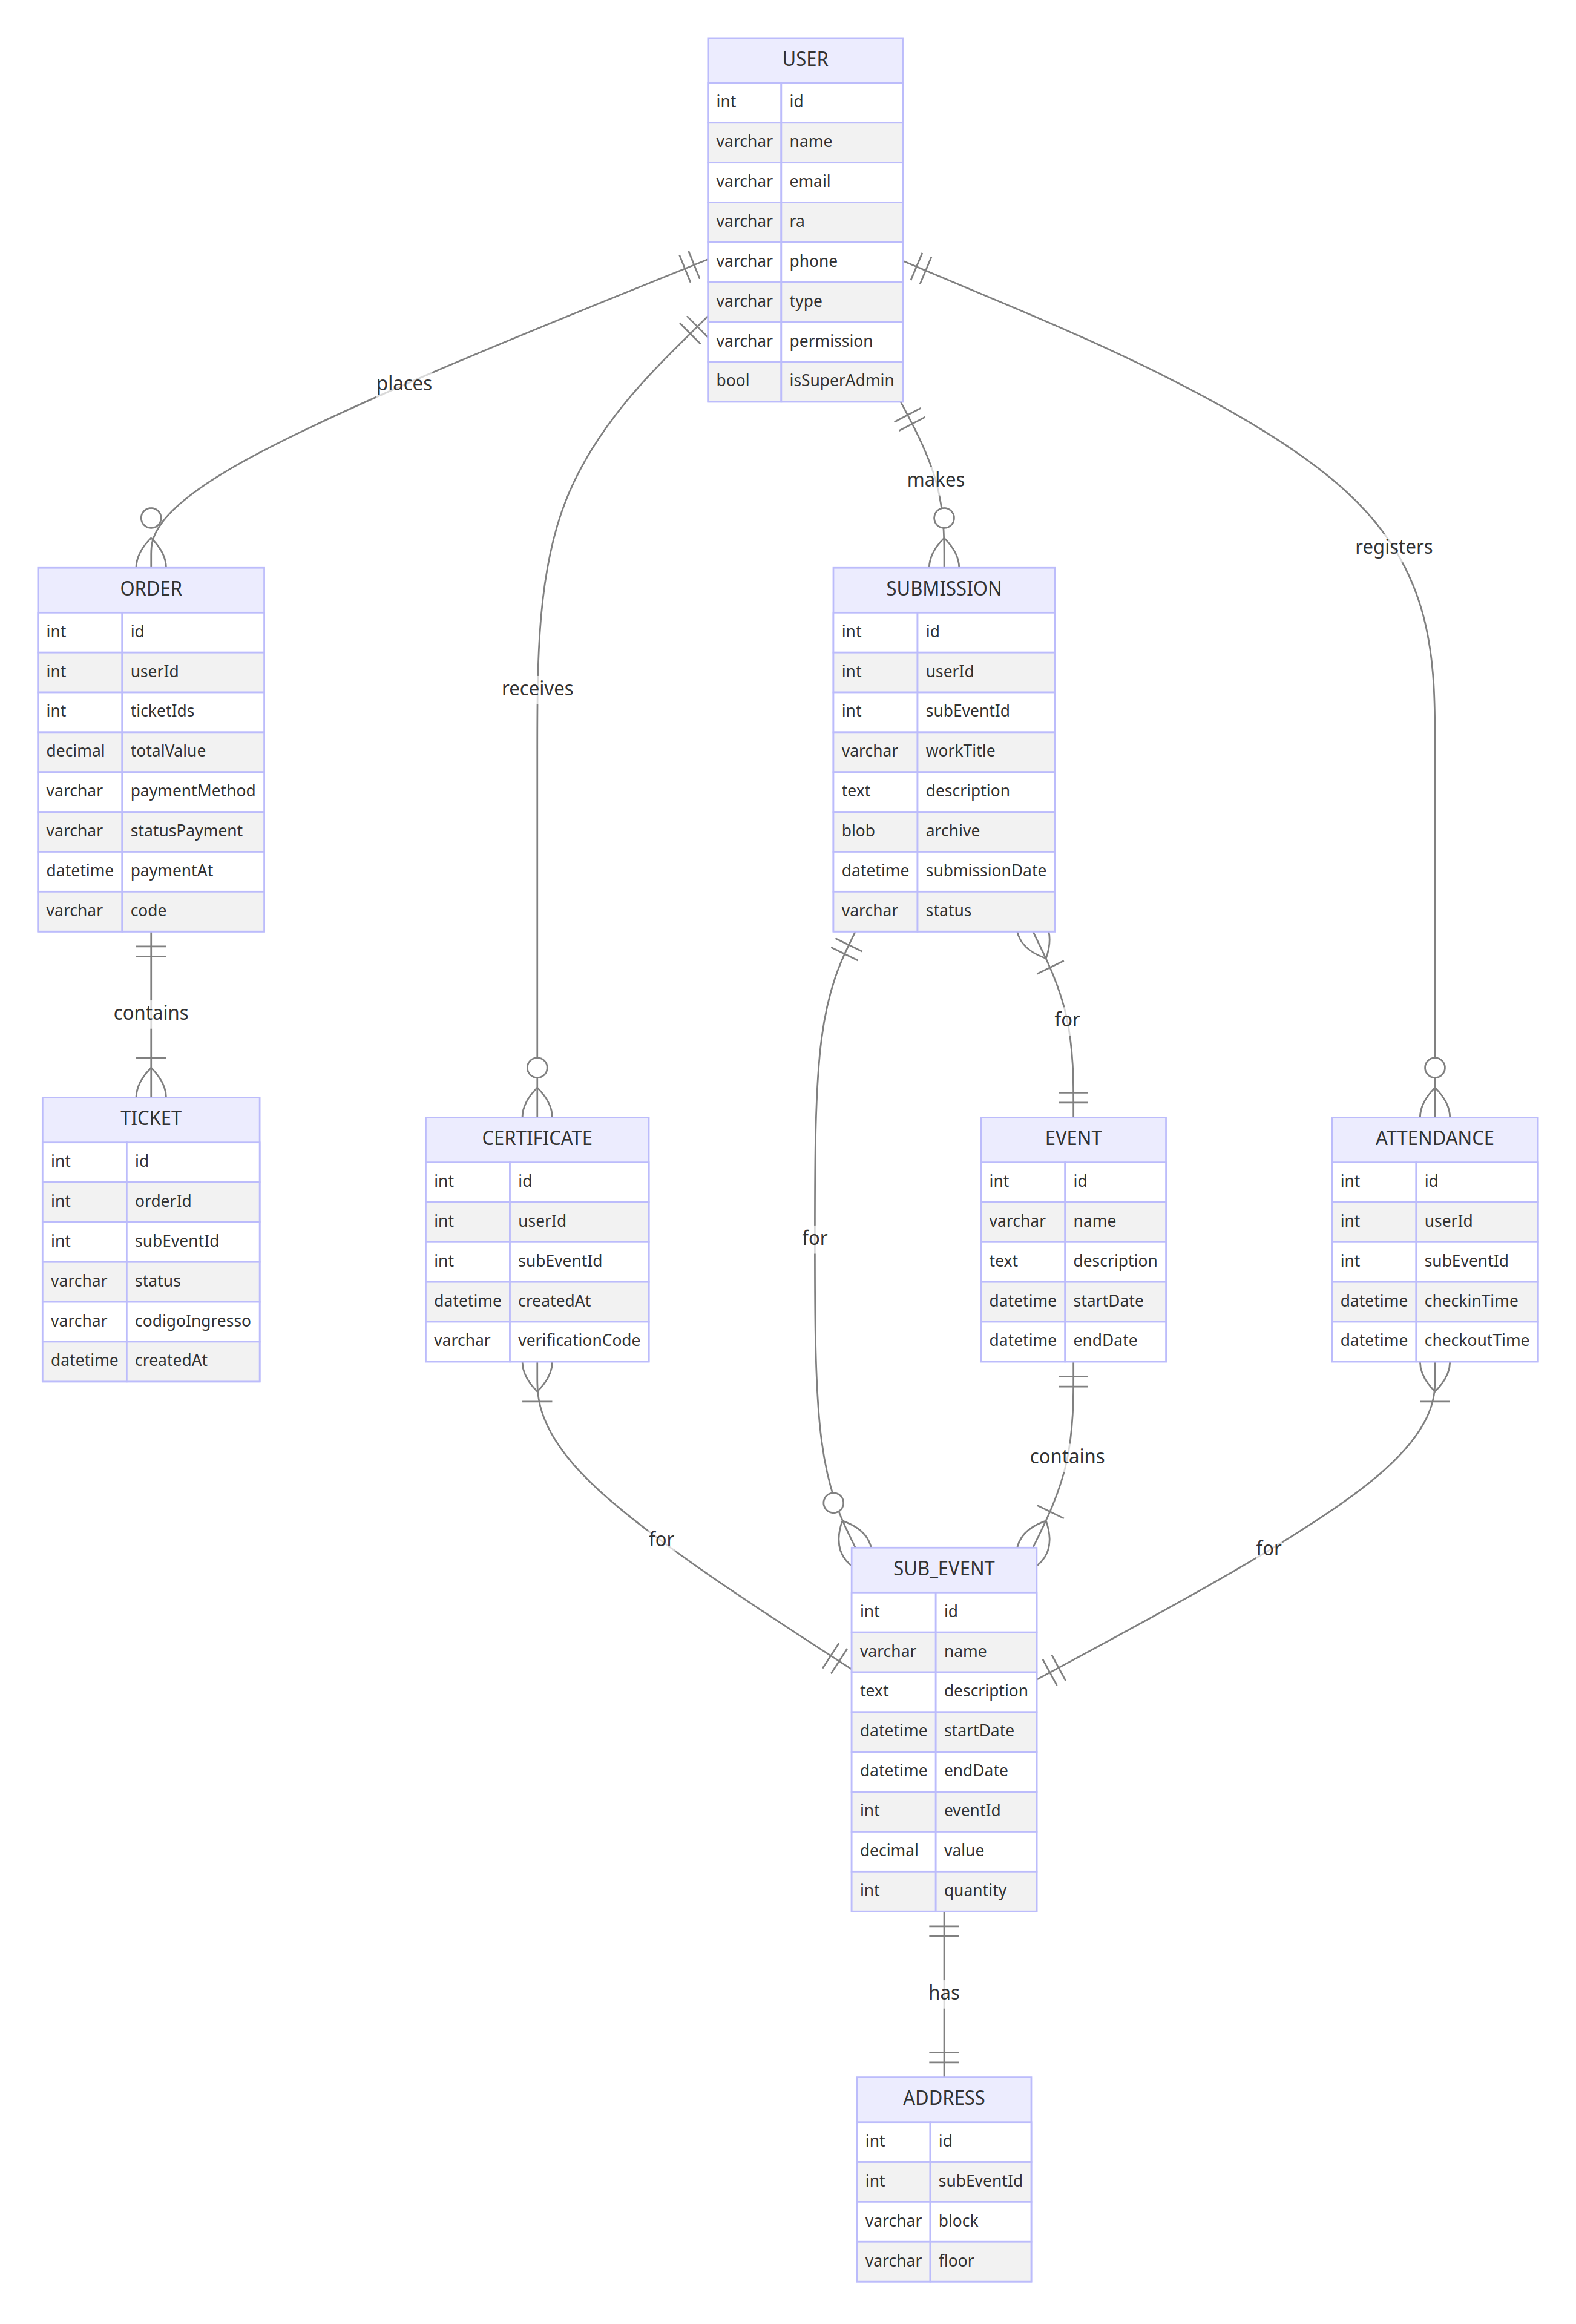
\includegraphics[width=0.8\textwidth]{figuras/diagrama-entidades.png}
\caption{Diagrama de Entidades do Sistema}
\label{fig:diagrama-entidades.png}
\end{figure}

\begin{verbatim}
erDiagram
    USER ||--o{ ORDER : places
    ORDER ||--|{ TICKET : contains
    USER ||--o{ CERTIFICATE : receives
    CERTIFICATE }|--|| SUB_EVENT : "for"
    USER ||--o{ SUBMISSION : makes
    SUBMISSION }|--|| EVENT : "for"
    SUBMISSION ||--o{ SUB_EVENT : "for"
    EVENT ||--|{ SUB_EVENT : contains
    SUB_EVENT ||--|| ADDRESS : has
    USER ||--o{ ATTENDANCE : registers
    ATTENDANCE }|--|| SUB_EVENT : "for"

    USER {
        int id
        varchar name
        varchar email
        varchar ra
        varchar phone
        varchar type
        varchar permission
        bool isSuperAdmin
    }

    ORDER {
        int id
        int userId
        int ticketIds
        decimal totalValue
        varchar paymentMethod
        varchar statusPayment
        datetime paymentAt
        varchar code
    }

    TICKET {
        int id
        int orderId
        int subEventId
        varchar status
        varchar codigoIngresso
        datetime createdAt
    }

    CERTIFICATE {
        int id
        int userId
        int subEventId
        datetime createdAt
        varchar verificationCode
    }

    SUBMISSION {
        int id
        int userId
        int subEventId
        varchar workTitle
        text description
        blob archive
        datetime submissionDate
        varchar status
    }

    EVENT {
        int id
        varchar name
        text description
        datetime startDate
        datetime endDate
    }

    SUB_EVENT {
        int id
        varchar name
        text description
        datetime startDate
        datetime endDate
        int eventId
        decimal value
        int quantity
    }

    ADDRESS {
        int id
        int subEventId
        varchar block
        varchar floor
    }

    ATTENDANCE {
        int id
        int userId
        int subEventId
        datetime checkinTime
        datetime checkoutTime
    }
\end{verbatim}

\section{Diagrama de Classes}

Abaixo está o diagrama de classes que ilustra a estrutura e os relacionamentos entre as entidades do sistema:

\begin{figure}[h]
\centering
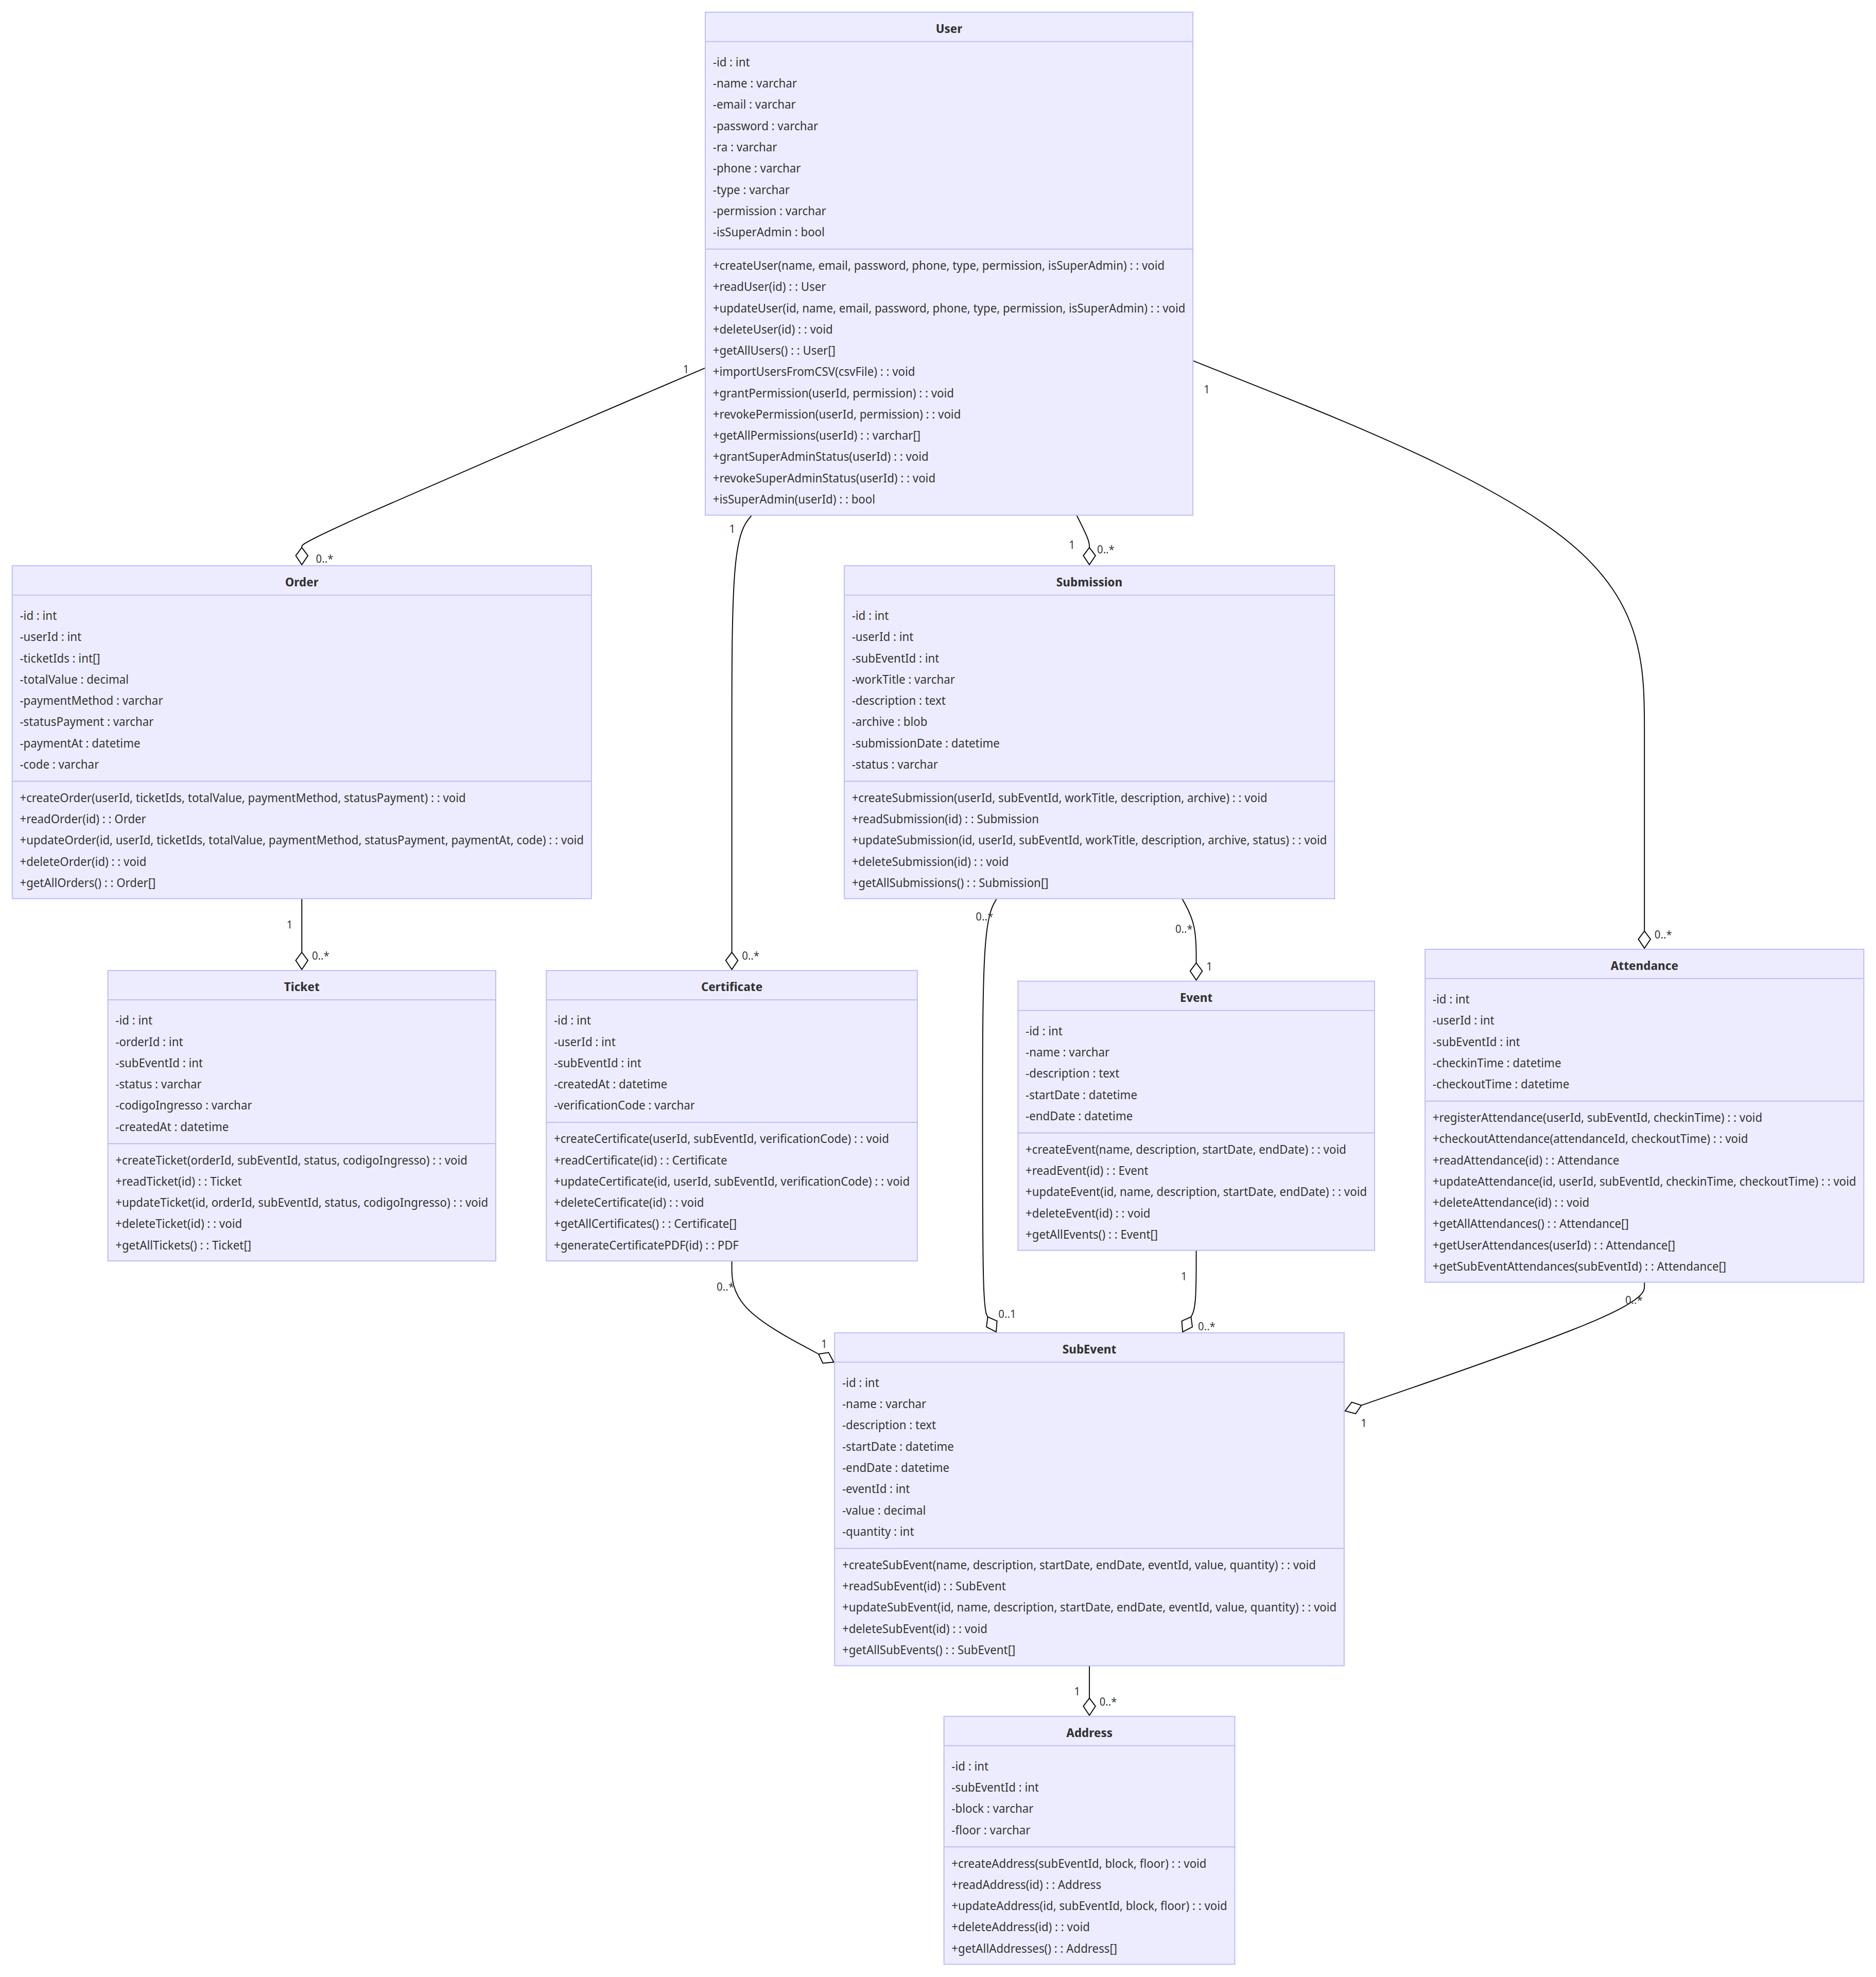
\includegraphics[width=0.8\textwidth]{figuras/diagrama-classes.png}
\caption{Diagrama de Classes do Sistema}
\label{fig:diagrama-classes}
\end{figure}

\begin{verbatim}
classDiagram
    class User {
        -id : int
        -name : varchar
        -email : varchar
        -password : varchar
        -ra : varchar
        -phone : varchar
        -type : varchar
        -permission : varchar
        -isSuperAdmin : bool
        +createUser(name, email, password, phone, type, permission, isSuperAdmin) : void
        +readUser(id) : User
        +updateUser(id, name, email, password, phone, type, permission, isSuperAdmin) : void
        +deleteUser(id) : void
        +getAllUsers() : User[]
        +importUsersFromCSV(csvFile) : void
        +grantPermission(userId, permission) : void
        +revokePermission(userId, permission) : void
        +getAllPermissions(userId) : varchar[]
        +grantSuperAdminStatus(userId) : void
        +revokeSuperAdminStatus(userId) : void
        +isSuperAdmin(userId) : bool
    }

    class Order {
        -id : int
        -userId : int
        -ticketIds : int[]
        -totalValue : decimal
        -paymentMethod : varchar
        -statusPayment : varchar
        -paymentAt : datetime
        -code : varchar
        +createOrder(userId, ticketIds, totalValue, paymentMethod, statusPayment) : void
        +readOrder(id) : Order
        +updateOrder(id, userId, ticketIds, totalValue, paymentMethod, statusPayment, paymentAt, code) : void
        +deleteOrder(id) : void
        +getAllOrders() : Order[]
    }

    class Ticket {
        -id : int
        -orderId : int
        -subEventId : int
        -status : varchar
        -codigoIngresso : varchar
        -createdAt : datetime
        +createTicket(orderId, subEventId, status, codigoIngresso) : void
        +readTicket(id) : Ticket
        +updateTicket(id, orderId, subEventId, status, codigoIngresso) : void
        +deleteTicket(id) : void
        +getAllTickets() : Ticket[]
    }

    class Certificate {
        -id : int
        -userId : int
        -subEventId : int
        -createdAt : datetime
        -verificationCode : varchar
        +createCertificate(userId, subEventId, verificationCode) : void
        +readCertificate(id) : Certificate
        +updateCertificate(id, userId, subEventId, verificationCode) : void
        +deleteCertificate(id) : void
        +getAllCertificates() : Certificate[]
        +generateCertificatePDF(id) : PDF
    }

    class Submission {
        -id : int
        -userId : int
        -subEventId : int
        -workTitle : varchar
        -description : text
        -archive : blob
        -submissionDate : datetime
        -status : varchar
        +createSubmission(userId, subEventId, workTitle, description, archive) : void
        +readSubmission(id) : Submission
        +updateSubmission(id, userId, subEventId, workTitle, description, archive, status) : void
        +deleteSubmission(id) : void
        +getAllSubmissions() : Submission[]
    }

    class Event {
        -id : int
        -name : varchar
        -description : text
        -startDate : datetime
        -endDate : datetime
        +createEvent(name, description, startDate, endDate) : void
        +readEvent(id) : Event
        +updateEvent(id, name, description, startDate, endDate) : void
        +deleteEvent(id) : void
        +getAllEvents() : Event[]
    }

    class SubEvent {
        -id : int
        -name : varchar
        -description : text
        -startDate : datetime
        -endDate : datetime
        -eventId : int
        -value : decimal
        -quantity : int
        +createSubEvent(name, description, startDate, endDate, eventId, value, 
        quantity) : void
        +readSubEvent(id) : SubEvent
        +updateSubEvent(id, name, description, startDate, endDate, eventId,
         value, quantity) : void
        +deleteSubEvent(id) : void
        +getAllSubEvents() : SubEvent[]
    }

    class Address {
        -id : int
        -subEventId : int
        -block : varchar
        -floor : varchar
        +createAddress(subEventId, block, floor) : void
        +readAddress(id) : Address
        +updateAddress(id, subEventId, block, floor) : void
        +deleteAddress(id) : void
        +getAllAddresses() : Address[]
    }

    class Attendance {
        -id : int
        -userId : int
        -subEventId : int
        -checkinTime : datetime
        -checkoutTime : datetime
        +registerAttendance(userId, subEventId, checkinTime) : void
        +checkoutAttendance(attendanceId, checkoutTime) : void
        +readAttendance(id) : Attendance
        +updateAttendance(id, userId, subEventId, checkinTime
        , checkoutTime) : void
        +deleteAttendance(id) : void
        +getAllAttendances() : Attendance[]
        +getUserAttendances(userId) : Attendance[]
        +getSubEventAttendances(subEventId) : Attendance[]
    }

    User "1" --o "0..*" Order
    Order "1" --o "0..*" Ticket
    User "1" --o "0..*" Certificate
    Certificate "0..*" --o "1" SubEvent
    User "1" --o "0..*" Submission
    Submission "0..*" --o "1" Event
    Submission "0..*" --o "0..1" SubEvent
    Event "1" --o "0..*" SubEvent
    SubEvent "1" --o "0..*" Address
    User "1" --o "0..*" Attendance
    Attendance "0..*" --o "1" SubEvent
\end{verbatim}
